\chapter{Hasil Studi}
\label{chap:hasilstudi}
Bab ini berisi hasil studi terhadap \textit{Business Process Model and Notation} dan \textit{Business Process Management System} Camunda. 

\section{Hasil Studi BPMN}
\label{sec:hasilstudi_bpmn}
Setiap bisnis memiliki alur kerja maupun proses yang perlu dilewati. Proses tersebut dapat digambarkan dalam bentuk \textit{Business Process Model and Notation}. BPMN merupakan sebuah standar untuk menggambarkan langkah-langkah pada suatu proses bisnis. Dengan BPMN, suatu proses bisnis yang kompleks dapat digambarkan menjadi lebih sederhana sehingga lebih mudah dimengerti. BPMN memiliki berbagai notasi seperti \textit{event, task, gateway, data, artifact, lanes}, dan \textit{pool}.  

	
\subsection{Masalah Proses Bisnis}
\label{hasilstudi_bpmn_masalah}
Berikut ini adalah dua contoh proses bisnis yang akan dimodelkan pada \textit{workflow} :
\begin{enumerate}
\item Pengajuan Proposal
Pegawai di perusahaan X memiliki tiga divisi yaitu \textit{accounting}, \textit{sales}, dan \textit{management}. Divisi \textit{accounting} dan \textit{sales} dapat mengajukan proposal bisnis ke divisi \textit{management}. Divisi \textit{management} harus memeriksa apakah proposalnya layak atau tidak. Jika proposalnya tidak layak, pembuat proposal harus memperbaiki dan mengunggahnya kembali. Apabila proposalnya layak, pegawai dapat melihat setelah status proposal tersebut. Workflow dari skenario ini sebagai berikut :


\item Proses Pendaftaran BPJS
\begin{enumerate}
	\item Pemohon mengisi formulir pendaftaran BPJS di situs BPJS (termasuk jenis keanggotaan).
	\item Pemohon mengupload semua dokumen persyaratan di situs BPJS.
	\item Sistem BPJS membangkitkan nomor pembayaran uang pendaftaran/ iuran pertama (nomor pembayaran selanjutnya menjadi nomor keanggotaan/ kartu BPJS).
  \item Pemohon melihat nomor pembayaran dan besarnya uang pendaftaran/ iuran pertama.
  \item Pemohon membayar uang pendaftaran/iuran pertama melalui bank sesuai nomor pembayaran.
  \item Pemohon memilih jadwal verifikasi dokumen asli yang tersedia.
  \item Sistem BPJS membangkitkan jadwal kedatangan dan nomor antrian.
  \item Pemohon mencetak jadwal kedatangan dan nomor antriannya.
  \item Pemohon datang ke kantor BPJS membawa dokumen asli (sesuai jadwal, jika tidak maka pendaftaran hangus). 
  \item Petugas BPJS memverifikasi pendaftaran, dan attachment dokumen persyaratan dan keasliannya. Jika valid dan lengkap, proses dilanjutkan ke langkah 11, jika tidak lengkap maupun tidak valid, maka kembali ke langkah 1.
	\item Sistem BPJS membangkitkan barcode untuk kartu BPJS.
  \item Petugas BPJS mencetak kartu BPJS dan meyerahkannya ke Pemohon.
\end{enumerate}

\end{enumerate}
		


\subsection{Memodelkan Proses Bisnis dengan \textit{Workflow}}
\label{hasilstudi_workflow}

\subsubsection{Pengajuan Proposal}
\label{workflow_kasus1}
Pada kasus Pengajuan Proposal, terdapat beberapa elemen, yaitu :
\begin{enumerate}
	\item Satu \textit{pool}, yaitu Pengajuan Proposal
	\item Dua \textit{lane}, yaitu lane untuk Pegawai dan Manajemen
	\item Dua \textit{event}, yaitu \textit{start event} (Ide Proposal) dan \textit{end event} Proposal Diterima
	\item Tiga \textit{user task}, yaitu Mengunggah Proposal oleh pegawai, Memeriksa Proposal oleh manajemen, dan Melihat Status Proposal oleh pegawai.
	\item Satu \textit{decision point}, yaitu penentuan apakah proposal layak atauk tidak
\end{enumerate}

	\begin{figure}[H]
			\centering
			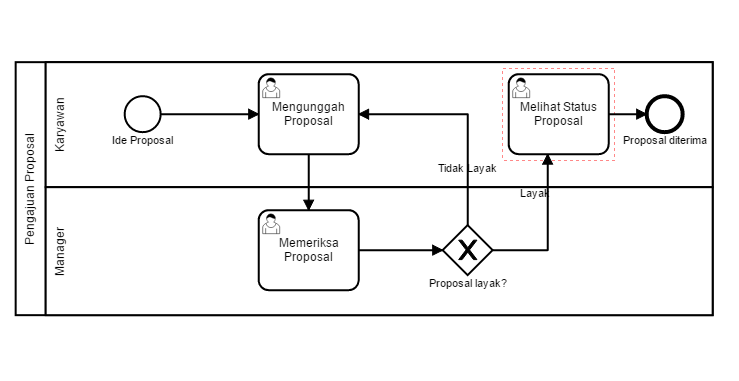
\includegraphics[scale=0.5]{Gambar/Bab-3/Kasus2-3}
			\caption{Mengunggah Proposal} 
			\label{fig:workflow_mengunggahproposal}
	\end{figure}
	
\begin{description}
	\item \textit{User task} Mengunggah Proposal dan Melihat Status Proposal\\
  \textit{Task} ini dapat dilakukan oleh pegawai (divisi \textit{sales} dan \textit{accounting}). Maka \textit{Candidate Groups} diisi dengan \textit{sales} dan \textit{accounting}.
		\begin{figure}[H]
			\centering
			
\includegraphics[scale=1]{Gambar/Bab-3/Kasus1/1group}
			\caption{Mengunggah Proposal} 
			\label{fig:pengajuanproposalmengunggahproposal_group}
	\end{figure}
	
	
	\item \textit{User task} Memeriksa Proposal
	
	 \textit{Task} ini dilakukan oleh Manajemen. Maka \textit{Candidate Groups} diisi dengan \textit{management}.
		\begin{figure}[H]
			\centering
			
\includegraphics[scale=1]{Gambar/Bab-3/Kasus1/3group2}
			\caption{Memeriksa Proposal} 
			\label{fig:pengajuanproposal_memeriksaproposal_group}
	\end{figure}
	


\end{description}


\subsubsection{Pendaftaran BPJS}
\label{workflow_kasus2}
Pada kasus Pendaftaran BPJS, terdapat beberapa elemen, yaitu :
\begin{enumerate}
	\item Satu \textit{pool}, yaitu Pendaftaran BPJS
	\item Empat \textit{lane}, yaitu lane untuk Pemohon (diwakilkan oleh John), Sistem BPJS, Petugas BPJS (diwakilkan oleh Mary) dan Petugas Bank (diwakilkan oleh Peter)
	\item Dua \textit{event}, yaitu \textit{start event} Membutuhkan BPJS dan \textit{end event} Pendaftaran Selesai
	\item Empat \textit{manual task} Pemohon, yaitu : 
			\begin{enumerate}
				\item Membuka situs BPJS
				\item Membayar uang pendaftaran sesuai nomor pembayaran
				\item Pergi ke kantor BPJS
				\item Menerima Kartu BPJS
			\end{enumerate}
	\item Tiga \textit{service task} Sistem BPJS, yaitu :
			\begin{enumerate}
				\item Membangkitkan nomor pembayaran dan uang pendaftaran
				\item Membangkitkan jadwal kedatangan dan nomor antrian
				\item Membangkitkan barcode untuk kartu BPJS
			\end{enumerate}
	\item Lima \textit{User task} Pemohon, yaitu :
			\begin{enumerate}
				\item Mengisi formulir pendaftaran BPJS
				\item Mengupload semua dokumen persyaratan
				\item Melihat nomor pembayaran dan besar uang pendaftaran 
				\item Memilih jadwal verifikasi dokumen
				\item Mencetak jadwal kedatangan dan nomor antrian
			\end{enumerate}
	\item Dua \textit{User task} Petugas BPJS, yaitu :
			\begin{enumerate}
				\item Memverifikasi pendaftaran dan \textit{attachment} dokumen persyaratan dan keaslian
				\item Mencetak kartu BPJS dan menyerahkannya
			\end{enumerate}
	\item Satu \textit{Manual task} Petugas Bank, yaitu menerima pembayaran
	\item Satu \textit{decision point}, yaitu penentuan apakah persyaratan pendaftaran lengkap dan valid
\end{enumerate}


		
		\begin{figure}[H]
			\centering
			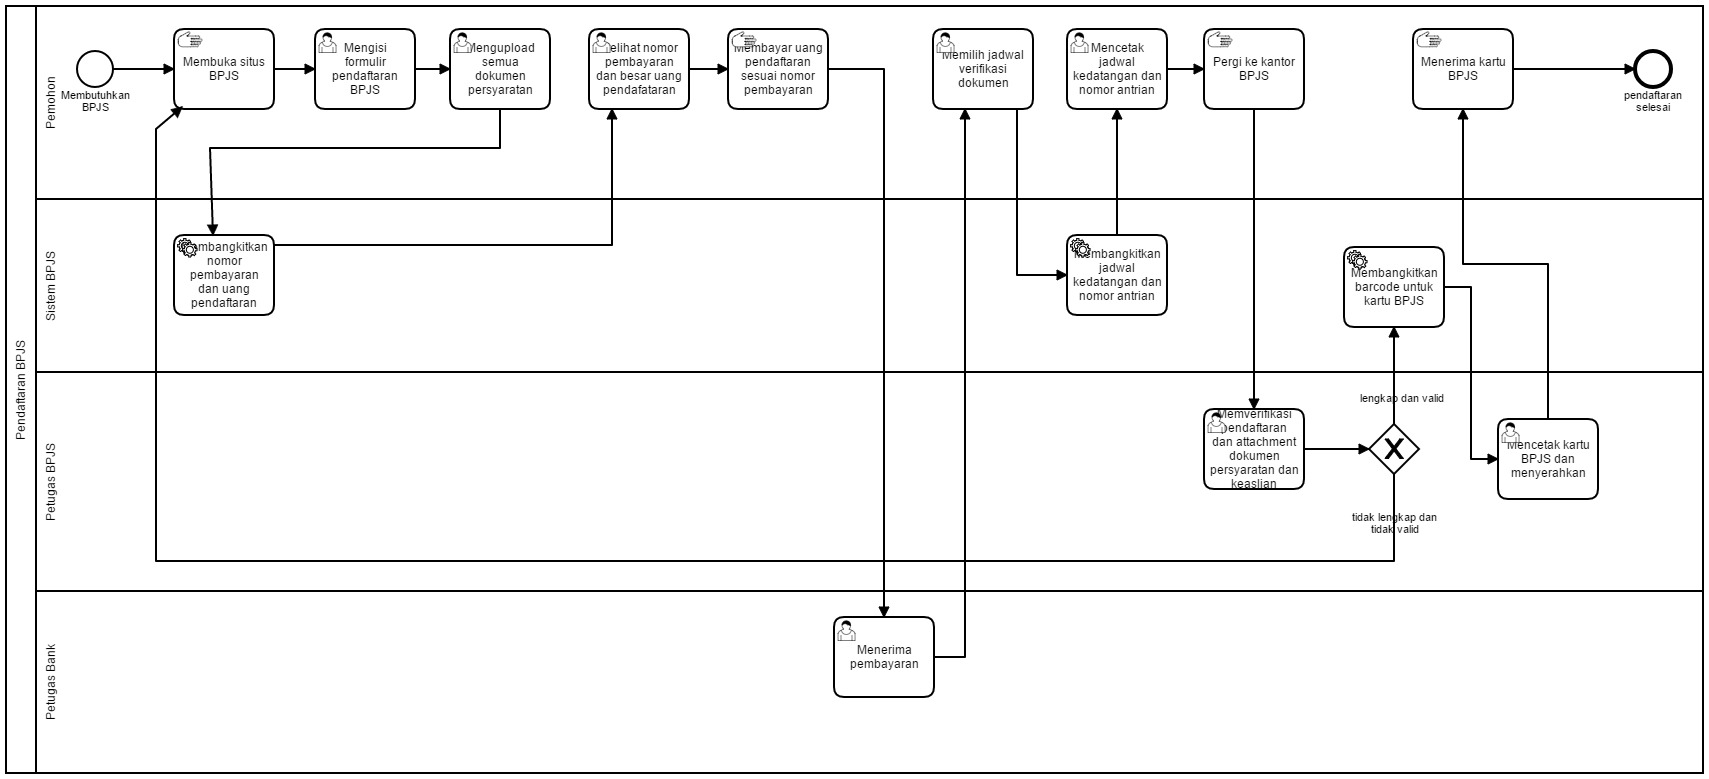
\includegraphics[scale=0.4 ,angle=90]{Gambar/Bab-3/Kasus2-4}
			\caption{Pendaftaran BPJS} 
			\label{fig:workflow_pendaftaranbpjs}
	\end{figure}

Untuk setiap \textit{user task}, ditentukan pemiliknya \textit{task} masing-masing. Pemohon diwakilkan oleh John, Petugas BPJS diwakilkan oleh Mary, dan Petugas Bank diwakilkan oleh Peter. Sehingga atribut assignee di setiap \textit{user task} akan diisi dengan john, mary, atau peter. Contohnya adalah \textit{task} Mengisi formulir pendaftaran BPJS yang dimiliki oleh John memiliki atribut \textit{assignee} john. 

	\begin{figure}[H]
			\centering
			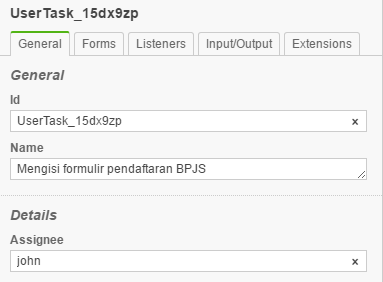
\includegraphics[scale=1]{Gambar/Bab-3/Kasus2/1assigneejohn}
			\caption{Atribut \textit{assignee} dari Mengisi formulir pendaftaran BPJS} 
			\label{fig:pendaftaranbpjs_assigneejohn}
	\end{figure}


\section{Menyiapkan BPMS Camunda}
\label{hasilstudi_menyiapkanbpms}
Bagian ini akan menjelaskan cara instalasi Camunda, menghungkan \textit{form} HTML maupun \textit{script} Java dengan BPMN, dan menjalankan otomasi proses bisnis menggunakan BPMS Camunda.
\subsection{Instalasi Camunda}
\label{hasilstudi_bpms_instalasicamunda}
Untuk menjalankan Camunda, diperlukan beberapa \textit{tool}\footnote{https://docs.camunda.org/get-started/bpmn20}, yaitu :
\begin{itemize}
	\item Java JDK 1.7+.
	\item Apache Maven atau Maven yang sudah terpasang di Eclipse.
	\item Web browser.
	\item Camunda BPM Platform 
	\item Camunda Modeler
\end{itemize}


\subsubsection{Mempersiapkan Proyek Java}
\begin{description}
	\item Membuat Proyek Maven di Eclipse. 
		\begin{enumerate}
			\item Pilih File / New / Other / Maven / Maven Project kemudian pilih \textit{Next}.
			\item Pilih Create a simple project (skip archetype selection) kemudian pilih \textit{next}.
			\item Pilih Packaging : war, kemudian pilih Finish.
		\end{enumerate}
	\item Tambahkan \textit{Camunda Maven Dependencies} ke file pom.xml (lihat Lampiran ~\ref{lamp:pom}).
	\item Tambahkan sebuah kelas Process Application pada direktori src/main/java. Nama kelas dapat diganti dengan nama proses yang dibuat. 
	\begin{lstlisting}[language=java,basicstyle=\tiny,caption=Kelas Process Application]
	package org.camunda.bpm.getstarted.loanapproval;

import org.camunda.bpm.application.ProcessApplication;
import org.camunda.bpm.application.impl.ServletProcessApplication;

@ProcessApplication("Loan Approval App")
public class LoanApprovalApplication extends ServletProcessApplication {
  // empty implementation
}
	\end{lstlisting}
	\item Tambahkan \textit{Deployment Descriptor} di META-INF/processes.xml.
	
	\begin{lstlisting}[language=xml,basicstyle=\tiny,caption=processes.xml]	
	<?xml version="1.0" encoding="UTF-8" ?>

<process-application
    xmlns="http://www.camunda.org/schema/1.0/ProcessApplication"
    xmlns:xsi="http://www.w3.org/2001/XMLSchema-instance">

  <process-archive name="loan-approval">
    <process-engine>default</process-engine>
    <properties>
      <property name="isDeleteUponUndeploy">false</property>
      <property name="isScanForProcessDefinitions">true</property>
    </properties>
  </process-archive>

</process-application>
	\end{lstlisting}
	
	
\end{description}

\subsection{Kasus 1 - Pengajuan Proposal}
\label{hasilstudi_bpms_kasus1}
Untuk menyiapkan proses bisnis pengajuan proposal sehingga dapat dijalankan oleh BPMS Camunda, langkah-langkah yang perlu dilakukan adalah :

\begin{enumerate}
	\item Menambah Form HTML untuk setiap \textit{user task} dan menghubungkannya dengan BPMN. File HTML yang dibuat disimpan di direktori src/main/webapp/forms. Proses bisnis ini memiliki dua \textit{user task}, yaitu mengunggah proposal dan memeriksa proposal. 
	
\begin{enumerate}
	\item \textit{User task} Mengunggah Proposal
	Task ini merupakan \textit{user task} sehingga membutuhkan suatu \textit{form} HTML untuk mengunggah proposal. Pada \textit{form} MengunggahProposal, isi dari variabel cam-variable-name adalah proposal yang akan digunakan pada \textit{form} tempat proposal diunduh.

	
	\begin{lstlisting}[language=html,basicstyle=\tiny,caption=MengunggahProposal.html]
		<html>
		<head></head>
		<body>
			<form method="post" name="upload-dokumen">
				<input type="file"
					 cam-variable-name="proposal" 
					 cam-variable-type="File"
					 cam-max-filesize="10000000"/>
			</form>
		</body>
		</html>
	\end{lstlisting}
	
		\begin{figure}[H]
			\centering
			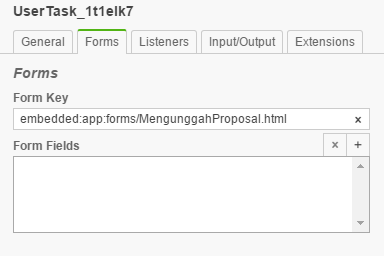
\includegraphics[scale=1]{Gambar/Bab-3/Kasus1/2form}
			\caption{Mengunggah Proposal} 
			\label{fig:pengajuanproposal_mengunggahproposalform}
	\end{figure}


\item \textit{User task} Memeriksa Proposal Task ini merupakan \textit{user task} sehingga membutuhkan suatu \textit{form} HTML untuk memeriksa proposal. Isi dari variabel cam-file-download adalah "proposal" (sama dengan cam-variable-name pada \textit{form} mengunggah proposal, sehingga file yang diunduh sama dengan file yang diunggah. Kemudian terdapat \textit{checkbox} untuk menentukan apakah proposal sudah layak atau belum. \textit{Checkbox} ini memiliki cam-variable-name dengan nama "valid" yang nantinya akan digunakan pada \textit{gateway}.

	
	\begin{lstlisting}[language=xml,basicstyle=\tiny,caption=MemeriksaProposal.html]
		<html>
		<head></head>
		<body>
		<form role="form" name="form">
				<a cam-file-download="proposal">Download Dokumen</a>
				<p>Apakah Proposal layak?</p>
				<input cam-variable-name="valid"
								 cam-variable-type="Boolean"
								 type="checkbox"
								 name="valid"
								 class="form-control" />		
		</form> 
		</body>
		</html>
	\end{lstlisting}
	
	\begin{figure}[H]
			\centering
			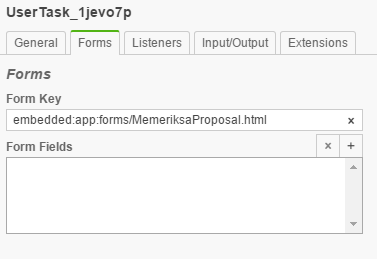
\includegraphics[scale=1]{Gambar/Bab-3/Kasus1/4form2}
			\caption{Memeriksa Proposal} 
			\label{fig:pengajuanproposal_memeriksaproposalhtml}
	\end{figure}

\item \textit{User Task} Melihat Status Proposal, pegawai dapat melihat status proposalnya apabila sudah diterima. Berikut adalah kodenya :
	\begin{lstlisting}[language=xml,basicstyle=\tiny,caption=MemeriksaProposal.html]
<html>
	<head></head>
	<body>
	<h> Proposal sudah diterima </h>
	
	<form role="form" name="form">
  	<a cam-file-download="proposal">Lihat Proposal</a>
  	</form>
	


</html>

	\end{lstlisting}

\end{enumerate}

\item Mengatur \textit{Gateway}, untuk mengatur keluaran dari \textit{gateway} pengaturan dapat dilakukan pada modeler dengan menggunakan cam-variable-name = valid pada checkbox di form MemeriksaProposal. Apabila proposal layak, maka \textit{expression} yang digunakan adalah \$(valid). Jika proposal tidak layak, \textit{expression} yang digunakan adalah \$(!valid).
		\begin{figure}[H]
			\centering
			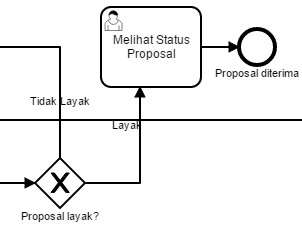
\includegraphics[scale=1]{Gambar/Bab-3/Kasus1/5layakgambar}
			\caption{Proposal Layak} 
			\label{fig:pengajuanproposal_layakgambar}
	\end{figure}
	\begin{figure}[H]
			\centering
			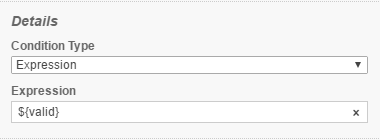
\includegraphics[scale=1]{Gambar/Bab-3/Kasus1/6layakkode}
			\caption{Ekspresi Proposal Layak} 
			\label{fig:pengajuanproposal_layakkode}
	\end{figure}
	
	\begin{figure}[H]
			\centering
			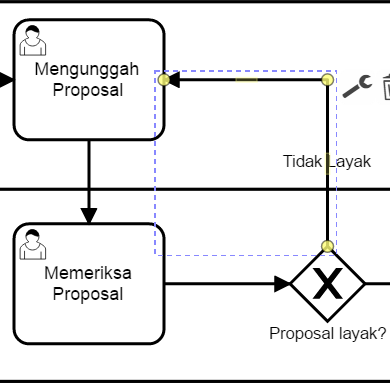
\includegraphics[scale=1]{Gambar/Bab-3/Kasus1/7tidaklayakgambar}
			\caption{Proposal tidak Layak} 
			\label{fig:pengajuanproposal_tidaklayakgambar}
	\end{figure}
	\begin{figure}[H]
			\centering
			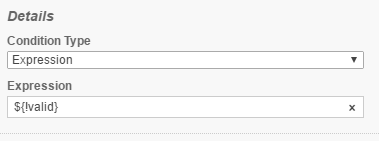
\includegraphics[scale=1]{Gambar/Bab-3/Kasus1/8tidaklayakkode}
			\caption{Ekspresi Proposal tidak Layak} 
			\label{fig:pengajuanproposal_tidaklayakkode}
	\end{figure}
	
	
	\item Menyimpan file BPMN ke direktori src/main/resources pada proyek pengajuan proposal
\end{enumerate}


\subsection{Kasus 2 - Pendaftaran BPJS}
\label{hasilstudi_bpms_kasus2}

Untuk menyiapkan proses bisnis pendaftaran BPJS sehingga dapat dijalankan oleh BPMS Camunda, langkah-langkah yang perlu dilakukan sedikit berbeda dengan proses bisnis pengajuan proposal, yaitu:

\begin{enumerate}
	\item Menambah Form HTML untuk setiap \textit{user task} dan menghubungkannya dengan BPMN. File HTML yang dibuat disimpan di direktori src/main/webapp/forms. 
	\item Menambah implementasi \textit{Service Task} menggunakan kode Java dan menghubungkannya dengan BPMN.
	\item Mengatur keluaran \textit{gateway}. 
	\item Menyimpan file BPMN ke direktori src/main/resources pada proyek pendaftaran BPJS.
\end{enumerate}

Bagian yang membedakan kasus ini dan kasus pengajuan proposal adalah sebagai berikut :
\begin{enumerate}
	\item Pengiriman dan penerimaan variabel dari satu form HTML ke form HTML lainnya. Contohnya adalah pemohon mendaftar BPJS pada form pendaftaran-bpjs.html kemudian variabel nama diambil di verifikasi-pendaftaran.html. Isi dari variabel cam-variable-name didaftarkan ke variabelManager (kumpulan variabel) dan diambil dengan fungsi fetchVariable('nama') pada form ringkasan-jadwal.html. Isi dari variabel nama ditempatkan menggunakan \$scope.nama dan <td>{{ nama }} menggunakan <table>.  Berikut adalah potongan kodenya :
	
	\begin{lstlisting}[language=html,basicstyle=\tiny,caption=pilih-jadwal.html]
	<form name="pendaftaranBPJS" role="form">
		<div class="control-group">
		<label class="control-label" for="nama">Nama</label>
	    <div class="controls">
	      <input id="nama"
	             class="form-control"
	             cam-variable-name = "nama"
	             cam-variable-type = "String"
	             type="text"
	             required>
	    </div>	
	</form>
	\end{lstlisting}
	
	\begin{lstlisting}[language=html,basicstyle=\tiny,caption=ringkasan-jadwal.html]
<form role="form" name="form">
	<script cam-script type="text/form-script">
    	camForm.on('form-loaded', function() {
	      camForm.variableManager.fetchVariable('nama');
	});
	camForm.on('variables-restored', function() {
		\$scope.nama = camForm.variableManager.variableValue('nama');
		});
  	</script>
		
	<table>
    <tr>
      <td>Nama:</td>
      <td>{{ nama }}</td> <!-- Lokasi variabel nama ditampilkan -->
    </tr>
	</table>
	\end{lstlisting}
	
			
	\item Tiga \textit{Service Task}, yaitu PembangkitBarcode, PembangkitJadwal, dan PembangkitNomor beserta pengiriman dan penerimaan variabel dari \textit{Service Task} ke form HTML maupun sebaliknya. Kelas PembangkitJadwal mengambil data jadwal yang dimasukkan pemohon pada form pilih-jadwal.html menggunakan perintah getVariable("jadwalHari"). Kelas ini juga membangkitkan nomor antrian secara acak. Variabel jadwal dan nomor antrian dikirimkan ke variableManager menggunakan perintah setVariable(). Berikut adalah potongan kode dari PembangkitJadwal.java
		
	\begin{lstlisting}[language=Java,basicstyle=\tiny,caption=PembangkitJadwal.java]
		public int nomorAntrian(){
			Random rand = new Random();
			int nomor = rand.nextInt(10);
			return nomor;
		}
	
	public void execute(DelegateExecution execution) throws Exception {
		execution.getVariable("jadwalHari");
		String jadwal = this.jadwalKedatangan(execution.getVariable("jadwalHari"));
		int nomor = this.nomorAntrian();

		execution.setVariable("jadwal", jadwal);
		execution.setVariable("nomor", nomor);
	}
	\end{lstlisting}
	
	\begin{lstlisting}[language=html,basicstyle=\tiny,caption=pilih-jadwal.html]
		<form>
		<select 
			cam-variable-name="jadwalHari"
			cam-variable-type="String"
	        cam-choices="jadwalHariPilihan"
	        >
		  		<option value="senin">Senin</option>
		  		<option value="selasa">Selasa</option>
		  		<option value="rabu">Rabu</option>
		  		<option value="kamis">Kamis</option>
		  		<option value="jumat">Jumat</option>
		</select>
	</form>
	\end{lstlisting}
	Untuk menambahkan kode Java ke BPMN, pilih \textit{implementation} Java Class pada modeler dan isi lokasi dari kelas Java tersebut. Contohnya sebagai berikut :
	
		\begin{figure}[H]
			\centering
			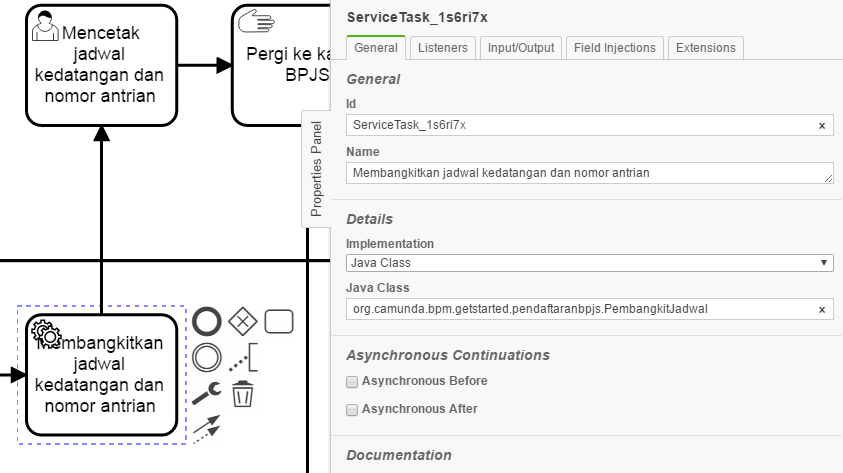
\includegraphics[scale=0.6]{Gambar/Bab-3/Kasus2/2servicetask}
			\caption{Menghubungkan \textit{Service Task} dengan kode Java} 
			\label{fig:pendaftaranBPJS_servicetask}
	\end{figure}
	
\end{enumerate}





\section{Menjalankan Camunda}
\label{hasilstudi_menjalankancamunda}
	\begin{enumerate}
		\item Klik kanan pom.xml dan pilih Run As / Maven Install. Langkah ini akan menghasilkan file WAR di folder target.
		\item \textit{Copy paste} file WAR ke CAMUNDA\_HOME / server / apache-tomcat / webapps folder.
		\item Jalankan start-camunda.bat
	\end{enumerate}
	
	
\subsection{Otomasi Kasus 1 - Pengajuan Proposal}
\label{menjalankancamunda_kasus1}	
Berikut adalah hasil otomasi kasus Pengajuan Proposal
\begin{enumerate}
	\item John, sebagai bagian dari divisi sales mengunggah proposal
	\begin{figure}[H]
			\centering
			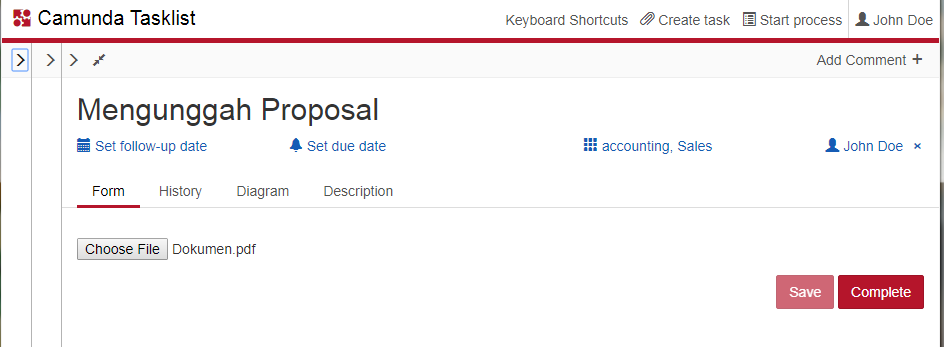
\includegraphics[scale=0.6]{Gambar/Bab-3/BPMS/Kasus1/1}
			\caption{Mengunggah Proposal} 
			\label{fig:otomasi_kasus1_1}
	\end{figure}
	\item Peter, sebagai bagian dari divisi manajemen memeriksa dan menyetujui proposal
	\begin{figure}[H]
			\centering
			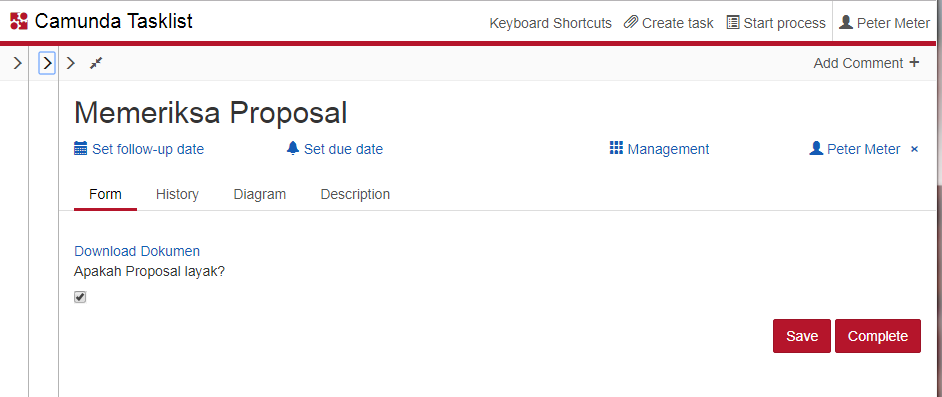
\includegraphics[scale=0.6]{Gambar/Bab-3/BPMS/Kasus1/2}
			\caption{Memeriksa Proposal} 
			\label{fig:otomasi_kasus1_2}
	\end{figure}
		\item John, sebagai bagian dari divisi sales melihat proposal telah disetujui
	\begin{figure}[H]
			\centering
			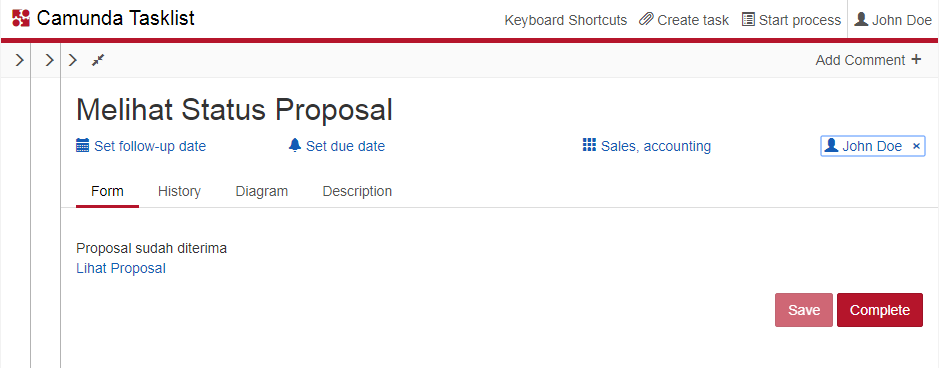
\includegraphics[scale=0.6]{Gambar/Bab-3/BPMS/Kasus1/3}
			\caption{Melihat Status Proposal} 
			\label{fig:otomasi_kasus1_3}
	\end{figure}
		
\end{enumerate}
		
		
\subsection{Otomasi Kasus 2 - Pendaftaran BPJS}
\label{menjalankancamunda_kasus2}
Berikut adalah hasil otomasi kasus Pendaftaran BPJS
\begin{enumerate}
	\item John mengisi data diri untuk mendaftar BPJS
	\begin{figure}[H]
			\centering
			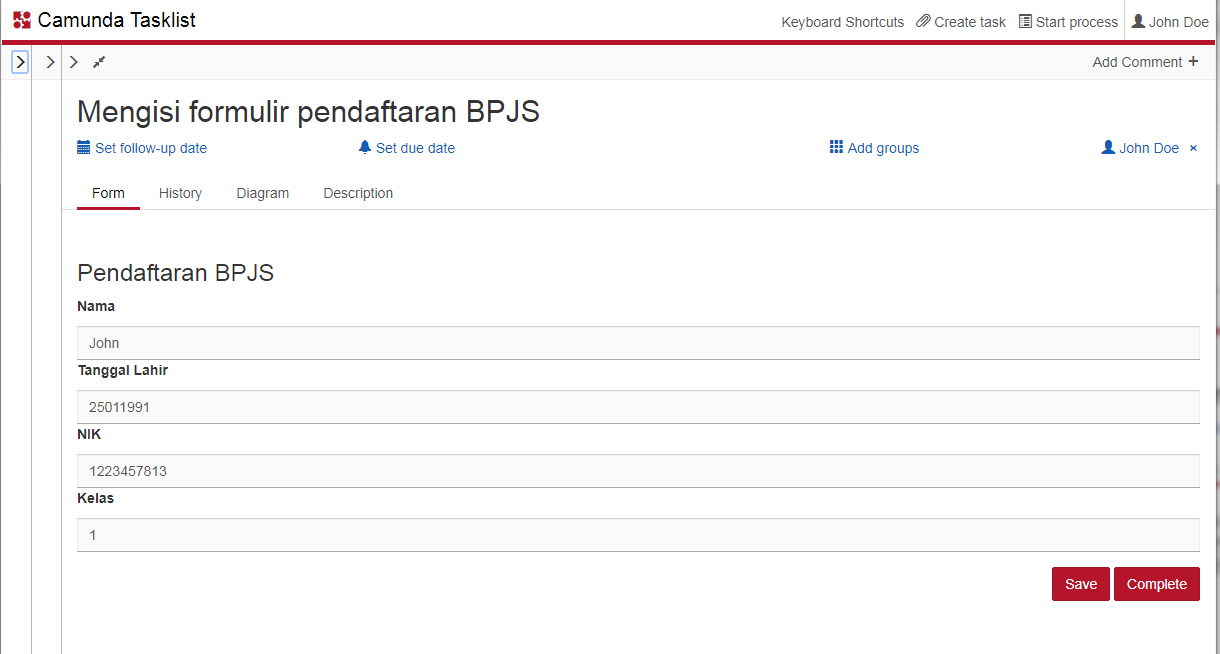
\includegraphics[scale=0.4]{Gambar/Bab-3/BPMS/Kasus2/1}
			\caption{Mendaftar BPJS} 
			\label{fig:otomasi_kasus2_1}
	\end{figure}
	
	\item John mengunggah semua dokumen persyaratan BPJS
	\begin{figure}[H]
			\centering
			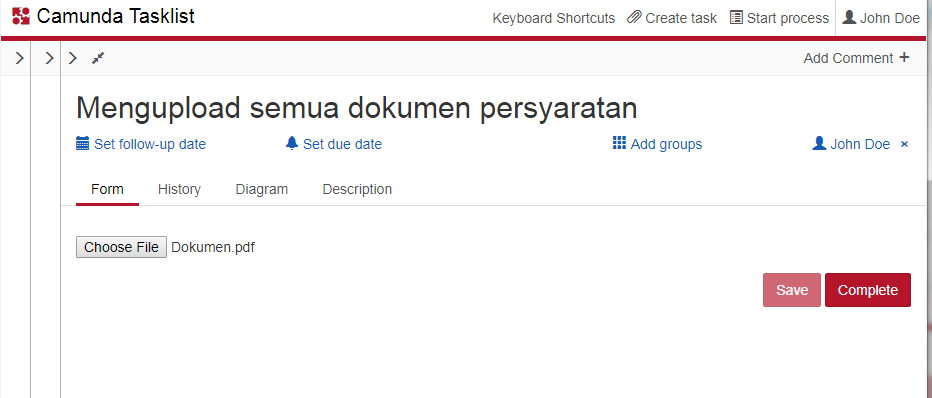
\includegraphics[scale=0.6]{Gambar/Bab-3/BPMS/Kasus2/2}
			\caption{Mengunggah Dokumen} 
			\label{fig:otomasi_kasus2_2}
	\end{figure}
	
	\item John melihat nomor pembayaran dan besar uang pendaftaran BPJS
	\begin{figure}[H]
			\centering
			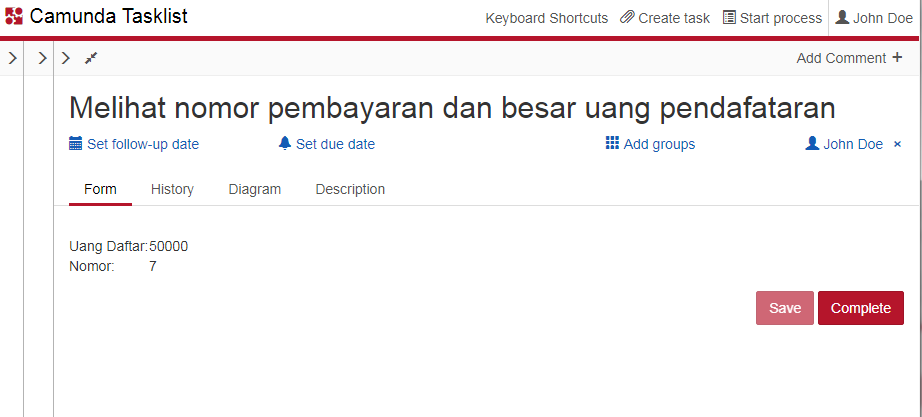
\includegraphics[scale=0.6]{Gambar/Bab-3/BPMS/Kasus2/3}
			\caption{Melihat Nomor dan Biaya Pendaftaran} 
			\label{fig:otomasi_kasus2_3}
	\end{figure}
	
	\item John memilih hari untuk verifikasi dokumen
	\begin{figure}[H]
			\centering
			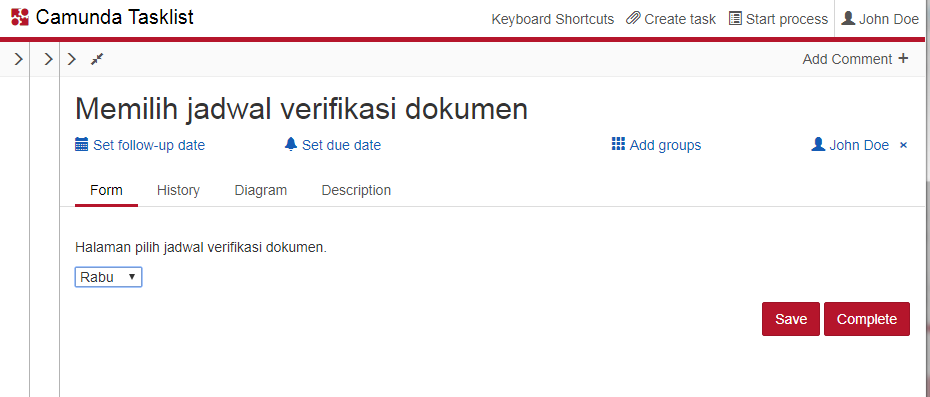
\includegraphics[scale=0.6]{Gambar/Bab-3/BPMS/Kasus2/4}
			\caption{Memilih Hari} 
			\label{fig:otomasi_kasus2_4}
	\end{figure}
	
	\item John Mencetak Jadwal Kedatangan dan Nomor Antrian
	\begin{figure}[H]
			\centering
			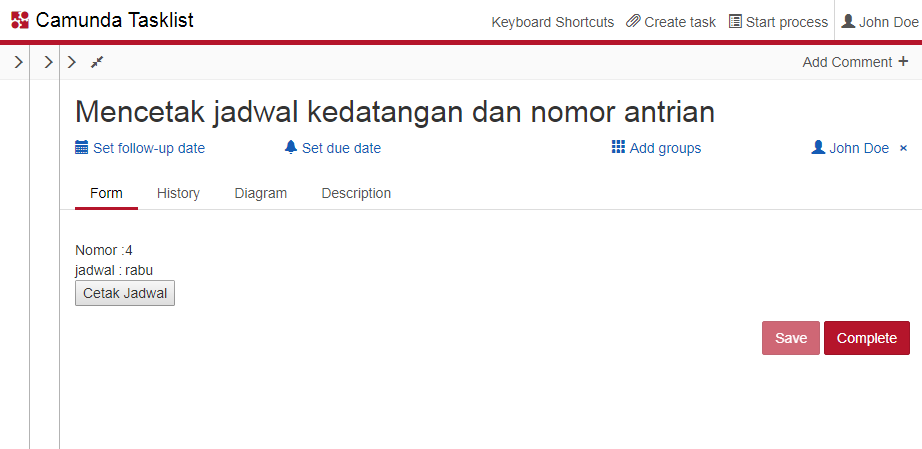
\includegraphics[scale=0.6]{Gambar/Bab-3/BPMS/Kasus2/5}
			\caption{Mencetak Jadwal} 
			\label{fig:otomasi_kasus2_5}
	\end{figure}
	
	\item Mary Memverifikasi pendaftaran BPJS
	\begin{figure}[H]
			\centering
			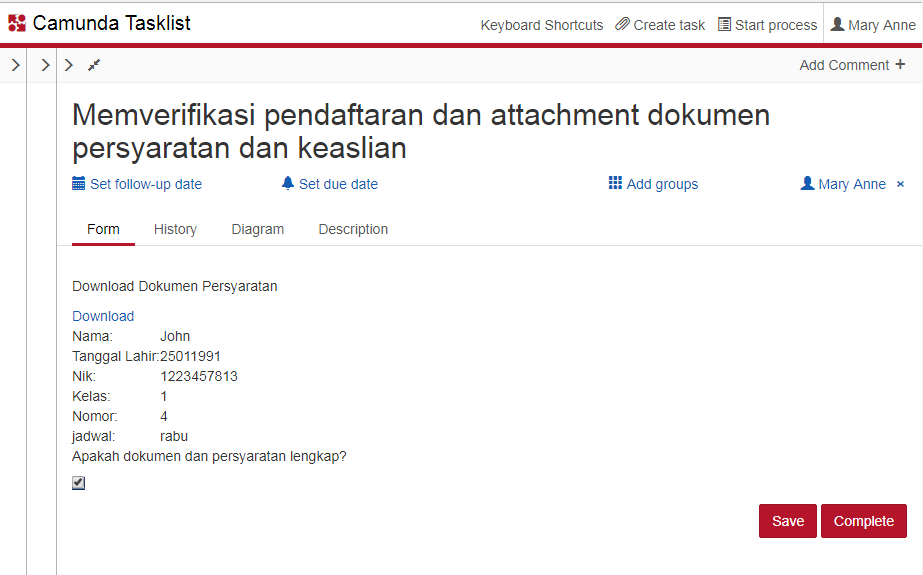
\includegraphics[scale=0.6]{Gambar/Bab-3/BPMS/Kasus2/6}
			\caption{Verifikasi Pendaftaran BPJS} 
			\label{fig:otomasi_kasus2_6}
	\end{figure}
	
	\item Mary Mencetak Kartu BPJS dan Menyerahkannya ke John
	\begin{figure}[H]
			\centering
			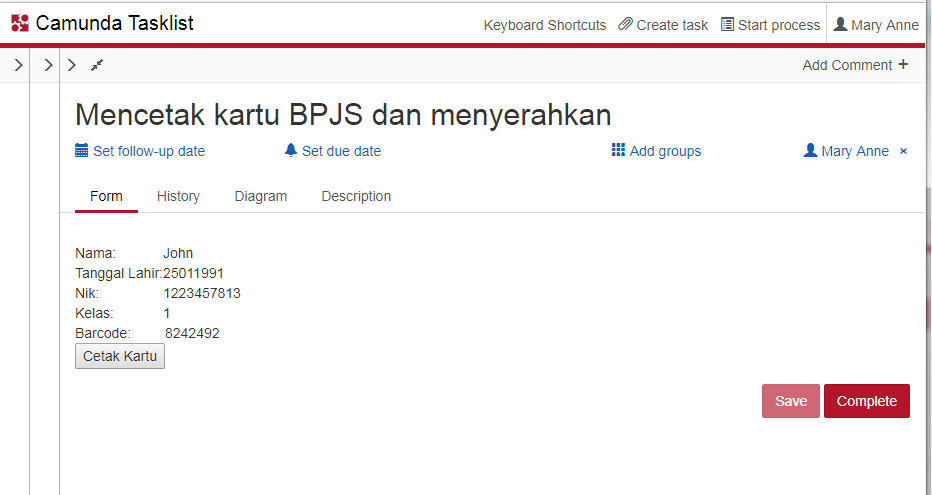
\includegraphics[scale=0.6]{Gambar/Bab-3/BPMS/Kasus2/7}
			\caption{Mencetak Kartu BPJS} 
			\label{fig:otomasi_kasus2_7}
	\end{figure}
	
\end{enumerate}

	